\chapter{Software Design and Requirements}
This section gives description about the requirements and the design of the project. It utilises DFDs(Data Flow Diagrams) to represent the working and inter-dependency of different modules of the system.
\section{System Requirements}
The major requirements for the system are listed below:
	\begin{itemize}
		\item Students are recognised by their faces and mapped to their IDs.
		\item Students can view their attended meals.
		\item Students get notified on entering the mess.
		\item Students can pay and view bills on monthly basis.
	\end{itemize}
\section{System Design}
System design shown in figure 3.1 is a representation of how different modules and users will interact with each other.
	\begin{figure}[!h]
    		\centering
    		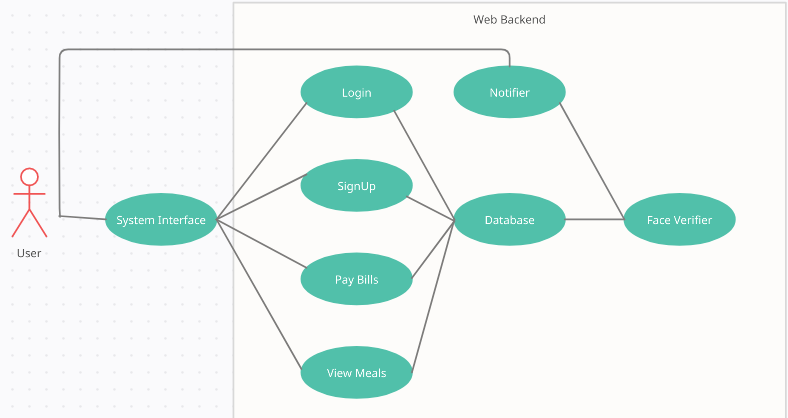
\includegraphics[width={\textwidth}]{Systemdesign}
    		\label{System Designo}
    		\caption{System Design}
	\end{figure}
\section{Data Flow Diagrams}
	\begin{itemize}
		\item Level 0 DFD: See figure 3.2
		\begin{figure}[!h]
    			\centering
    			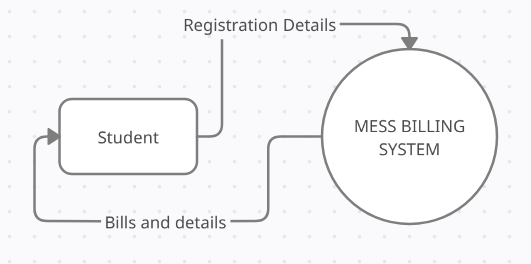
\includegraphics[width={\textwidth}]{Level0DFD}
    			\caption{Level 0 DFD}
		\end{figure}
		\item Level 1 DFD: See figure 3.3
		\begin{figure}[!h]
    			\centering
    			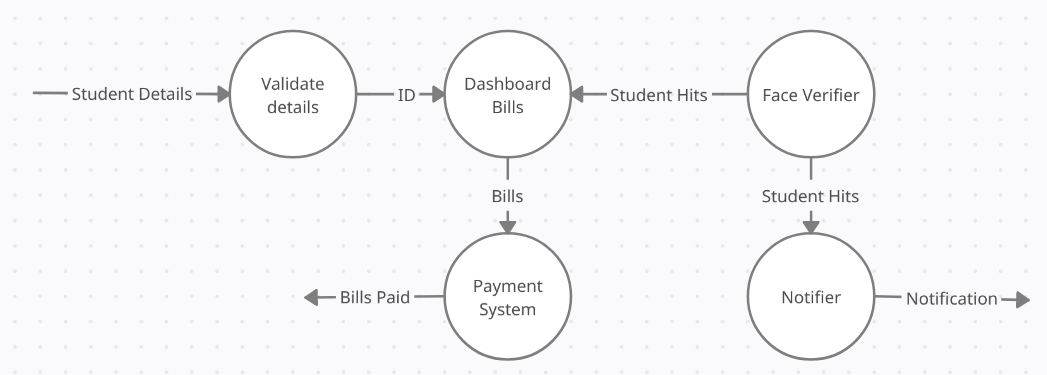
\includegraphics[width={\textwidth}]{Level1DFD}
    			\caption{Level 1 DFD}
		\end{figure}
		\item Level 2 DFD: See figure 3.4
		\begin{figure}[!h]
    			\centering
    			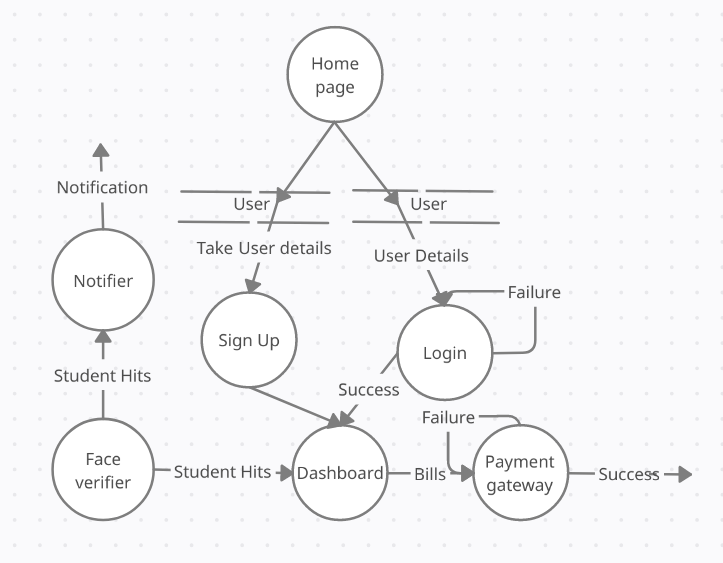
\includegraphics[width={\textwidth}]{Level2DFD}
    			\caption{Level 2 DFD}
		\end{figure}
	\end{itemize}
\section{Implementation specifics}
This sub-section proposes the tech-stack used in the project.
	\begin{itemize}
		\item \textbf{Pytorch} : It is used as the framework for development of face recognition model.
		\item \textbf{MERN stack} : MERN stands for MongoDB database, Express.JS, React.JS, Node.JS.  This is the used stack for web interface.
		\item \textbf{requests} : It is a module in python used for making calls to web server from face recognition system.
		\item \textbf{Twilio API} : This is the Application Programming Interface(API) used to send notification messages to students.
		\item \textbf{Payment gateway} : It will be an API used to allow students pay their bills online. We are yet to choose which API to use. The deciding factors for the chosen API will be latency, cost effectiveness, and, ease of use.
	\end{itemize}
\section{Conclusion}
This section was a representation of system design and interface using Data Flow Diagrams. This will help me to develop things more precisely. Also, the addition of new features would be more straightforward.
